% ex: ts=2 sw=2 sts=2 et filetype=tex
% SPDX-License-Identifier: CC-BY-SA-4.0


\section{BIOS, UEFI/EFI}

\begin{frame}[c]{¿Qué es la BIOS?}
  \begin{columns}
    \column{0.3\textwidth}
      \begin{center}
        \includegraphics[scale=1.0]{lfs/amiBIOS.jpg}
      \end{center}
    \column{0.7\textwidth}
    \begin{itemize}
      \item El sistema básico de entrada-salida o \textbf{BIOS}
        (del inglés \textbf{Basic Input/Output System}) es un estándar de
        facto que define la interfaz de \textbf{firmware} para computadoras
        IBM PC compatibles.
      \pausa
      \item El firmware del BIOS es instalado dentro de la computadora
        personal (PC), y es el primer programa que se ejecuta cuando se
        \emph{enciende la computadora}.
      \pausa
      \item El propósito fundamental del BIOS es \textbf{iniciar}, y
        \textbf{probar el hardware} del sistema y cargar un \emph{gestor de
        arranque} o un sistema operativo desde un dispositivo de
        almacenamiento de datos.
    \end{itemize}
  \end{columns}
\end{frame}

\begin{frame}[c]{¿Qué es un firmware?}
  \begin{itemize}
    \item El \textbf{firmware} o \textbf{soporte lógico inalterable} es u
      programa informático que establece la lógica de más \emph{bajo nivel}
      que controla los \emph{circuitos electrónicos} de un dispositivo de
      cualquier tipo.
    \pausa
    \item Está fuertemente integrado con la electrónica del dispositivo.
    \pausa
    \item Un \emph{firmware} es un software que maneja físicamente al
      \textbf{hardware}.
  \end{itemize}
\end{frame}

\begin{frame}[c]{¿Qué es la UEFI/EFI?}
  \begin{columns}
    \column{0.4\textwidth}
      \begin{center}
        \includegraphics[scale=0.45]{lfs/uefi_pila.png}
      \end{center}
    \column{0.6\textwidth}
    \begin{itemize}
      \item La \textbf{Unified Extensible Firmware Interface} (UEFI, "interfaz
        unificada de firmware extensible" en español) es una especificación
        que define una interfaz entre el sistema operativo y el firmware.
    \end{itemize}
  \end{columns}
\end{frame}

\begin{frame}[c]{¿Qué es la UEFI/EFI?}
  \begin{columns}
    \column{0.3\textwidth}
      \begin{center}
        \includegraphics[scale=0.5]{lfs/uefi.png}
      \end{center}
    \column{0.7\textwidth}
    \begin{itemize}
      \item UEFI reemplaza la antigua interfaz del Sistema Básico de Entrada
        y Salida (BIOS) estándar presentado en las computadoras personales
        IBM PC como IBM PC ROM BIOS.
      \pausa
      \item La interfaz UEFI incluye \textbf{bases de datos} con información
        de la plataforma, \textbf{inicio y tiempo de ejecución} de los
        servicios disponibles listos para cargar el sistema operativo.
    \end{itemize}
  \end{columns}
\end{frame}

\begin{frame}[c]{Unified Extensible Firmware Interface}
  UEFI destaca principalmente por:
    Diseño modular.
  \begin{itemize}
    \item Compatibilidad y emulación del BIOS para los sistemas operativos
      solo compatibles con esta última.
    \pausa
    \item Soporte completo para la \textbf{Tabla de particiones GUID} (GPT),
      se pueden crear hasta 128 particiones por disco, con una capacidad
      total de 8 ZB.
    \pausa
    \item Capacidad de arranque desde unidades de almacenamiento grandes,
      dado que no sufren de las limitaciones del MBR.
    \pausa
    \item Independiente de la arquitectura y controladores de la CPU.
    \pausa
    \item Entorno amigable y flexible Pre-Sistema Operativo, incluyendo
      capacidades de red.
  \end{itemize}
\end{frame}

\begin{frame}[c]{Unified Extensible Firmware Interface}
  La EFI hereda las nuevas características avanzadas del BIOS como
  \textbf{ACPI} (Interfaz Avanzada de Configuración y Energía) y el
  \textbf{SMBIOS} (Sistema de Gestión de BIOS), y se le pueden añadir
  muchas otras, ya que el entorno se ejecuta en \textbf{64 bits} y no en
  16 bits, como su predecesora.
\end{frame}

\section{Arranque y tabla de particiones}

\begin{frame}[c]{Tabla de particiones}
  \begin{itemize}
    \item Una tabla de particiones es un \textbf{índice} que divide el
      espacio de almacenamiento en distintas secciones, llamadas
      particiones.
    \pausa
    \item Da ciertas características de cada partición, como por ejemplo
      el sistema de ficheros usado en ella o si la partición es arrancable,
      de solo lectura, etc.
    \pausa
    \item Hay distintos alternativas para definir la tabla de particiones:
      \pausa
      \begin{itemize}
        \item Tabla de particiones en el MBR, también llamada tabla de
          particiones DOS. Usada en IBM PC y compatibles con sistemas BIOS.
        \pausa
        \item GUID Partition Table. Propuesta por la especificación EFI y
          permite ser usada por IBM PC y compatibles con BIOS y con UEFI.
        \pausa
        \item Apple Partition Map (APM)
        \item Sun partition table (BSD disklabel)
        \item SGI (IRIX) partition table
      \end{itemize}
  \end{itemize}
\end{frame}

\begin{frame}[c]{Partición de disco}
  \begin{center}
    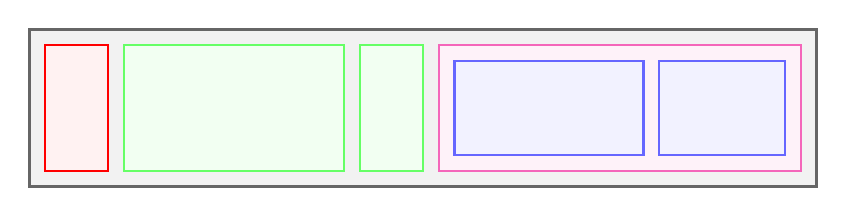
\begin{tikzpicture}
      \draw[draw=black!60, fill=black!5, very thick] (0,0) rectangle (10,2);
      \draw[draw=red, fill=red!5, thick] (0.2,0.2) rectangle (1,1.8);
      \draw[draw=green!60, fill=green!5, thick] (1.2,0.2) rectangle (4,1.8);
      \draw[draw=green!60, fill=green!5, thick] (4.2,0.2) rectangle (5,1.8);
      \draw[draw=magenta!60, fill=magenta!5, thick] (5.2,0.2) rectangle (9.8,1.8);
      \draw[draw=blue!60, fill=blue!5, thick] (5.4,0.4) rectangle (7.8,1.6);
      \draw[draw=blue!60, fill=blue!5, thick] (8,0.4) rectangle (9.6,1.6);
    \end{tikzpicture}
  \end{center}
  \begin{itemize}
    \item Una \textbf{partición de un disco duro} es una \textbf{división
      lógica} en una unidad de almacenamiento (por ejemplo, un disco duro o
      unidad flash),
    \pausa
    \item Se alojan y organizan los archivos mediante un \textbf{sistema de
    archivos}.
    \pausa
    \item Existen distintos esquemas de particiones para la distribución de
      particiones en un disco. Los más conocidos y difundidos son
      \textbf{MBR} (Master Boot Record) y \textbf{GPT} (GUID Partition Table).
  \end{itemize}
\end{frame}

\begin{frame}[c]{Tabla de particiones tipo MBR o DOS}
  En el esquema de particiones \textbf{MBR} o \textbf{DOS} existen 3 tipos
  diferentes de \textbf{particiones}:

  \pausa
  \vspace{\baselineskip}
  \begin{description}
    \item[primaria] Son las divisiones crudas o primarias del disco,
      solo puede haber como máximo 4 de éstas o 3 primarias y una extendida.
    \pausa
    \item[extendida] También conocida como partición secundaria es
      otro tipo de partición que actúa como una partición primaria; sirve
      ara contener múltiples unidades lógicas en su interior.
    \pausa
    \item[lógica] Ocupa una porción de la partición extendida o la
      totalidad de la misma, la cual se ha formateado con un tipo específico
      de sistema de archivos y se le ha asignado una unidad, así el sistema
      operativo reconoce las particiones lógicas o su sistema de archivos.
  \end{description}
\end{frame}

\begin{frame}[c]{Tabla de particiones tipo MBR o DOS}
  \begin{center}
    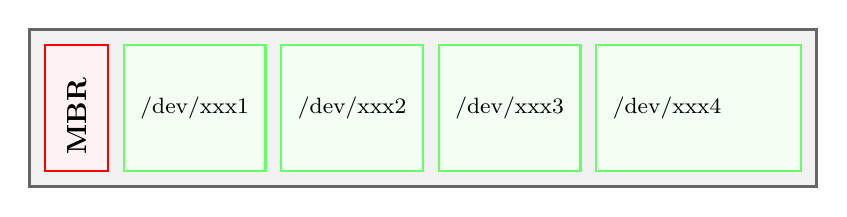
\begin{tikzpicture}
      \draw[draw=black!60, fill=black!5, very thick] (0,0) rectangle (10,2);
      \draw[draw=red, fill=red!5, thick] (0.2,0.2) rectangle (1,1.8);
      \node[rotate=90] at (0.6,0.9) {\textbf{MBR}};
      \draw[draw=green!60, fill=green!5, thick] (1.2,0.2) rectangle (3,1.8);
      \draw[draw=green!60, fill=green!5, thick] (3.2,0.2) rectangle (5,1.8);
      \draw[draw=green!60, fill=green!5, thick] (5.2,0.2) rectangle (7,1.8);
      \draw[draw=green!60, fill=green!5, thick] (7.2,0.2) rectangle (9.8,1.8);
      \node at (2.1,1) {\footnotesize{/dev/xxx1}};
      \node at (4.1,1) {\footnotesize{/dev/xxx2}};
      \node at (6.1,1) {\footnotesize{/dev/xxx3}};
      \node at (8.1,1) {\footnotesize{/dev/xxx4}};
    \end{tikzpicture}
  \end{center}
  \pausa
  \begin{center}
    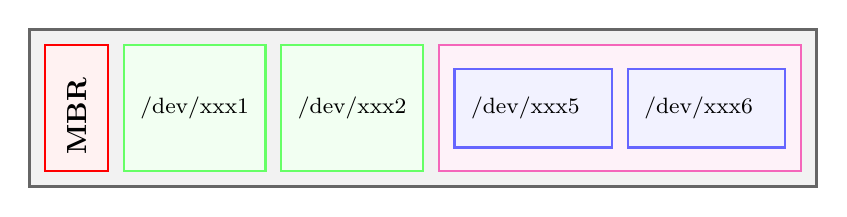
\begin{tikzpicture}
      \draw[draw=black!60, fill=black!5, very thick] (0,0) rectangle (10,2);
      \draw[draw=red, fill=red!5, thick] (0.2,0.2) rectangle (1,1.8);
      \node[rotate=90] at (0.6,0.9) {\textbf{MBR}};
      \draw[draw=green!60, fill=green!5, thick] (1.2,0.2) rectangle (3,1.8);
      \draw[draw=green!60, fill=green!5, thick] (3.2,0.2) rectangle (5,1.8);
      \draw[draw=magenta!60, fill=magenta!5, thick] (5.2,0.2) rectangle (9.8,1.8);
      \draw[draw=blue!60, fill=blue!5, thick] (5.4,0.5) rectangle (7.4,1.5);
      \draw[draw=blue!60, fill=blue!5, thick] (7.6,0.5) rectangle (9.6,1.5);
      \node at (2.1,1) {\footnotesize{/dev/xxx1}};
      \node at (4.1,1) {\footnotesize{/dev/xxx2}};
      \node at (6.3,1) {\footnotesize{/dev/xxx5}};
      \node at (8.5,1) {\footnotesize{/dev/xxx6}};
    \end{tikzpicture}
  \end{center}
  \pausa
  \begin{center}
    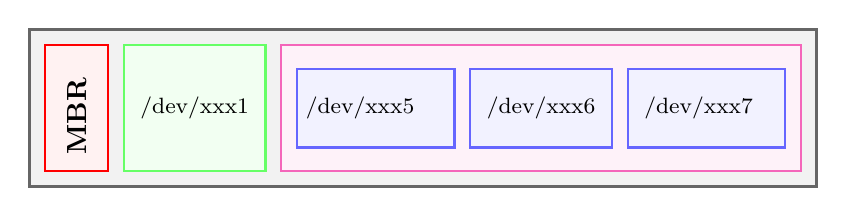
\begin{tikzpicture}
      \draw[draw=black!60, fill=black!5, very thick] (0,0) rectangle (10,2);
      \draw[draw=red, fill=red!5, thick] (0.2,0.2) rectangle (1,1.8);
      \node[rotate=90] at (0.6,0.9) {\textbf{MBR}};
      \draw[draw=green!60, fill=green!5, thick] (1.2,0.2) rectangle (3,1.8);
      \draw[draw=magenta!60, fill=magenta!5, thick] (3.2,0.2) rectangle (9.8,1.8);
      \draw[draw=blue!60, fill=blue!5, thick] (3.4,0.5) rectangle (5.4,1.5);
      \draw[draw=blue!60, fill=blue!5, thick] (5.6,0.5) rectangle (7.4,1.5);
      \draw[draw=blue!60, fill=blue!5, thick] (7.6,0.5) rectangle (9.6,1.5);
      \node at (2.1,1) {\footnotesize{/dev/xxx1}};
      \node at (4.2,1) {\footnotesize{/dev/xxx5}};
      \node at (6.5,1) {\footnotesize{/dev/xxx6}};
      \node at (8.5,1) {\footnotesize{/dev/xxx7}};
    \end{tikzpicture}
  \end{center}
\end{frame}

\begin{frame}[c]{MBR: Master Boot Record}
  Un \textbf{registro de arranque principal}, conocido también como
  \textbf{registro de arranque maestro} (por su nombre en inglés
  \textbf{master boot record}, MBR) es el
  primer sector de un dispositivo de almacenamiento de datos, como un disco
  duro.

  \vspace{\baselineskip}
  El MBR casi siempre se refiere al sector de arranque de \textbf{512 bytes},
  o el \textbf{partition sector} de una partición para ordenadores
  compatibles con IBM PC.

  \vspace{\baselineskip}
  \begin{center}
    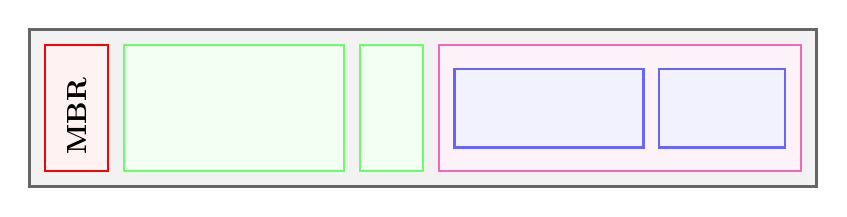
\begin{tikzpicture}
      \draw[draw=black!60, fill=black!5, very thick] (0,0) rectangle (10,2);
      \draw[draw=red, fill=red!5, thick] (0.2,0.2) rectangle (1,1.8);
      \node[rotate=90] at (0.6,0.9) {\textbf{MBR}};
      \draw[draw=green!60, fill=green!5, thick] (1.2,0.2) rectangle (4,1.8);
      \draw[draw=green!60, fill=green!5, thick] (4.2,0.2) rectangle (5,1.8);
      \draw[draw=magenta!60, fill=magenta!5, thick] (5.2,0.2) rectangle (9.8,1.8);
      \draw[draw=blue!60, fill=blue!5, thick] (5.4,0.5) rectangle (7.8,1.5);
      \draw[draw=blue!60, fill=blue!5, thick] (8,0.5) rectangle (9.6,1.5);
    \end{tikzpicture}
  \end{center}
\end{frame}

\begin{frame}[c]{Tabla de particiones GUID: GPT}

\end{frame}

\section{Sistemas de archivos}

\begin{frame}[c]{Sistemas de archivos}

\end{frame}

\begin{frame}[c]{Volúmenes Lógicos}

\end{frame}

\section{Sistemas de almacenamiento}

\begin{frame}[fragile]
  \frametitle{Sintaxis}
  %\begin{lstlisting}[language=Bash]
  %\end{lstlisting}

  \vspace{\baselineskip}
\end{frame}
